\section{Selection of crystals for SCXRD}

	The criteria for selection of crystals for SCXRD is as follows:%
%			
		\begin{itemize}%
%			
		    \item \bfnt{Uniform internal structure}: The crystal should not have more than one domain of array of unit cells, should not be composed of a number of micron or sub-micron sized particles, and should not have crack or distortion of any means. However, \ifnt{the crystal need not have well defined faces}.
		    
		    \item \bfnt{Suitable size and shape}: For SCXRD experiments, chosen crystals should have dimensions in the range $50-500~\si{\micro\metre}.$ The size of the crystal must be smaller than the spot size of the X-ray beam.
		    
		    \begin{figure}
		    	\centering
		    	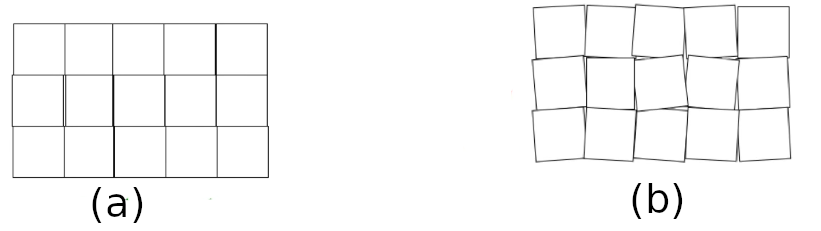
\includegraphics[scale=0.5]{imperfect_crystal.png}
		    	\caption{\label{fig:imperfect_crystal}The crystal on the left is a perfect crystal. The one on the right is a mosaic crystal with a deviation of $\sim 0.1-0.2 \si{\degree}.$}
		    \end{figure}
		    
		    \item \bfnt{Imperfect crystals are better.} In perfect crystals, lattice planes traverse in the whole crystal without any deviation, resulting into extinction. Majority of crystals are imperfect, and they diffract better than perfect crystals. Imperfectness may be deliberately introduced into a crystal by a shock.
		    
		    \begin{figure}
		    	\centering
		    	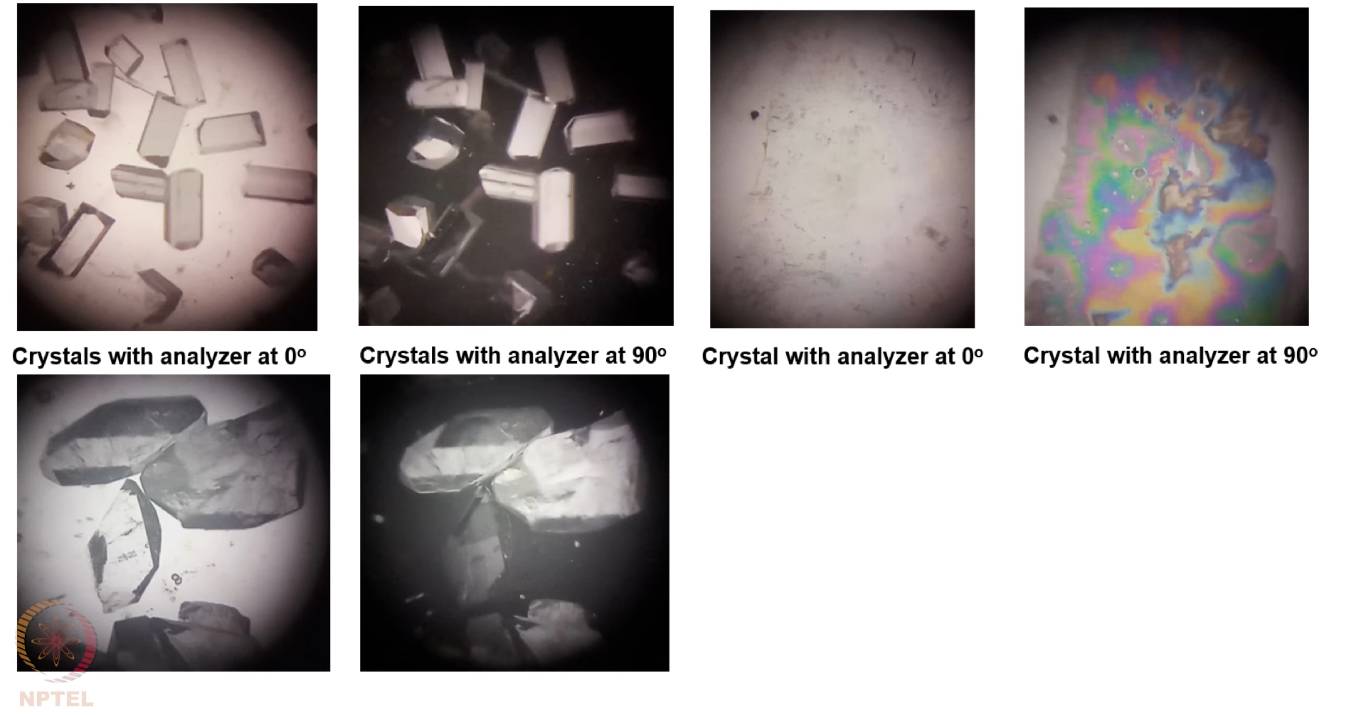
\includegraphics[scale=0.4]{crystal_optical_microscope.png}
		    	\caption{\label{fig:crystal_optical_micro}Crystals when viewed through an optical microscope in polarized light. The set of crystals on the left are good crystals because they are either uniformly dark or uniformly bright when the analyzer is rotated by $\pi/2.$ The crystal on the right shows different colours when the analyzer is rotated, implying that it has more than one domain and cannot be studied under SCXRD.}
		    \end{figure}
		    
		    \item \bfnt{Screening under optical microscope for domains}: Polarized light is passed through a crystal, and the crystal is rotated about its axis. The transmitted light is observed through an analyzer. If, on rotating the analyzer, the crystals appears either uniformly dark or uniformly bright in all regions of the crystal, then the crystal has a single domain. Crystals with multiple domains would appear both dark and bright, or show multiple colours at certain angles between the polarizer and analyzer. This is demonstrated in figure~\ref{fig:crystal_optical_micro}.
		    
		\end{itemize}

	We cannot know whether a crystal is good or bad until we mount it on the diffractometer and put it in the path of X-rays. Therefore, when a crystal passes the above minimum selection criteria, we mount it on the goniometer head and shine X-rays on it. The axis about which the crystal is mounted is known as the $\phi$ axis. We rotate crystal about the $\phi$ axis through a full $2\pi$ rotation while keeping the X-ray on for 1-2 minutes depending on the size of the crystal, and we keep recording the diffraction pattern. The diffraction pattern thus recorded is known as the \bfnt{rotation photograph} of the single crystal.
	
	\begin{figure*}
		\centering
		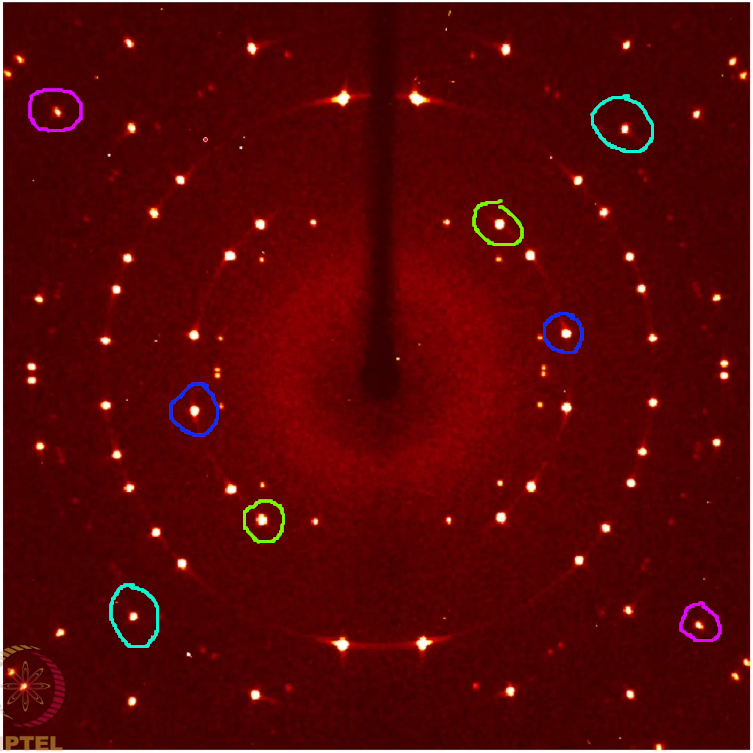
\includegraphics[scale=0.3]{rotation_photograph_mod.png}
		\caption{\label{fig:rotation_photo}Rotation photograph of a single crystal. Each spot has another spot on the other side related by a centre of inversion. Some examples are shown by different coloured circles; two spots encircled by the same colour are related to each other. The dark shadow is that of the beam stop, which prevents the direct X-ray beam from falling on the detector.}
	\end{figure*}
	
	Figure~\ref{fig:rotation_photo} shows the rotation photograph of a single crystal. This photograph is always centro-symmetric irrespective of the type of crystal geometry. Each spot on the rotation photograph has another corresponding spot that is related to it by a centre of inversion. If instead of these spots, the rotation photograph is composed of concentric circles, we conclude that the crystal is not a single crystal, but a polycrystal, and is not suitable for XRD.